\section{Methods}

In order to demonstrate that the DISHTINY platform selects for detectable hierarchical transitions in individuality, we performed experiments where cells controlled by evolving genetic programs evolved open-ended behaviors to make decisions about resource sharing, reproductive timing, and apoptosis.
We will first cover the design of the DISHTINY platform and then describe the cell-like organisms we used to evaluate the platform.

\subsection{Same-Channel Groups}

DISHTINY allows cell-like organisms to replicate across a toroidal grid.
Over discrete time steps (``updates''), the cells can collect a continuous-valued resource.
Once sufficient resource has been accrued, cells may pay $1.0$ resource to place a daughter cell on an adjoining tile of the toroidal grid (i.e., reproduce), replacing any existing cell already there.
Collected resource decays at a rate of 0.1\% per update, incentivizing its quick use.

Cells may benefit from a cooperative resource-collection process conducted by explicitly-registered ``signaling channel'' groupings.
As cells reproduce, they can choose to include offspring in the parent's cooperating ``signaling channel'' group or expel offspring to found a new cooperating ``signaling channel'' group.
These decisions affect the spatial layout of these ``signaling channel'' groups and, in turn, affect individual cells' resource-collection rate.
Medium-size, circular ``signaling channel'' groups tend to collect resource at a greater per-cell rates than large, small, ovular, or irregularly distributed groups.
In order to promote group turnover, we counteract the advantage of established group with a simple aging scheme.
As channel groups age over elapsed updates and elapsed somatic generations, their constituent cells lose the ability regenerate somatic tissue and then, soon after, to collect resource

A complete description of the mechanisms behind these collective resource-collection and group aging mechanisms appears in supplementary materials \ref{sup:resource_collection_process} \ref{sup:channel_group_life_cycle}.

In addition to a potentially functionally cooperative relationship, shared channel IDs --- which may only systematically arise through inheritance --- imply a close hereditary relationship.
In this work, we screen for fraternal transitions in individuality with respect to these same-channel network groups by evaluating resource sharing, antagonistic cell proliferation, and apoptosis across within-group and between-group contexts.

\subsection{Cell-Level Organisms}

\begin{figure}
\begin{center}

\hspace*{\fill}%
\begin{minipage}[t]{\columnwidth}
\centering
\vspace{0pt} % for alignment
\begin{subfigure}[b]{\textwidth}
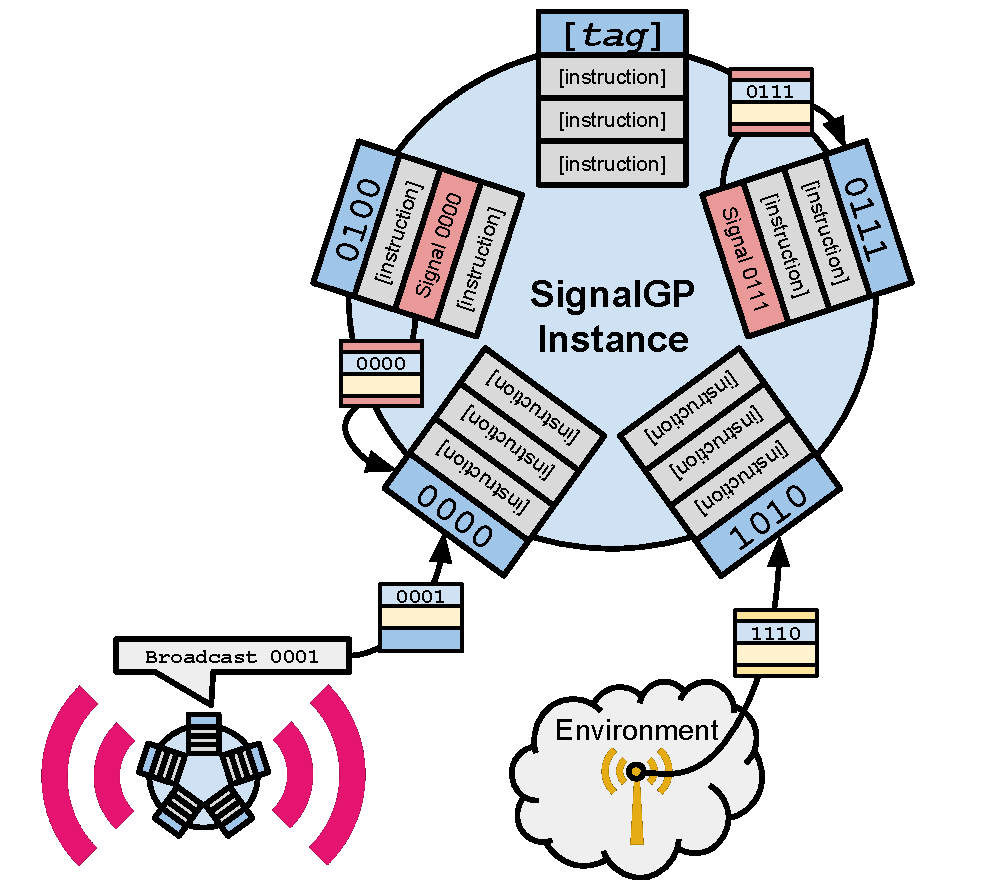
\includegraphics[width=\textwidth]{img/signalgp-cartoon}%
\caption{
A cartoon overview of a single SignalGP instance.
SignalGP program modules execute pseudo-concurrently in response to tagged signals, which can originate internally, from the environment, or from other agents.
}
\label{fig:signalgp-cartoon}
\end{subfigure}
\end{minipage}%
\hspace*{\fill}

\hspace*{\fill}%
\begin{minipage}[t]{\columnwidth}
\centering
\vspace{0pt} % for alignment
\begin{subfigure}[b]{\textwidth}
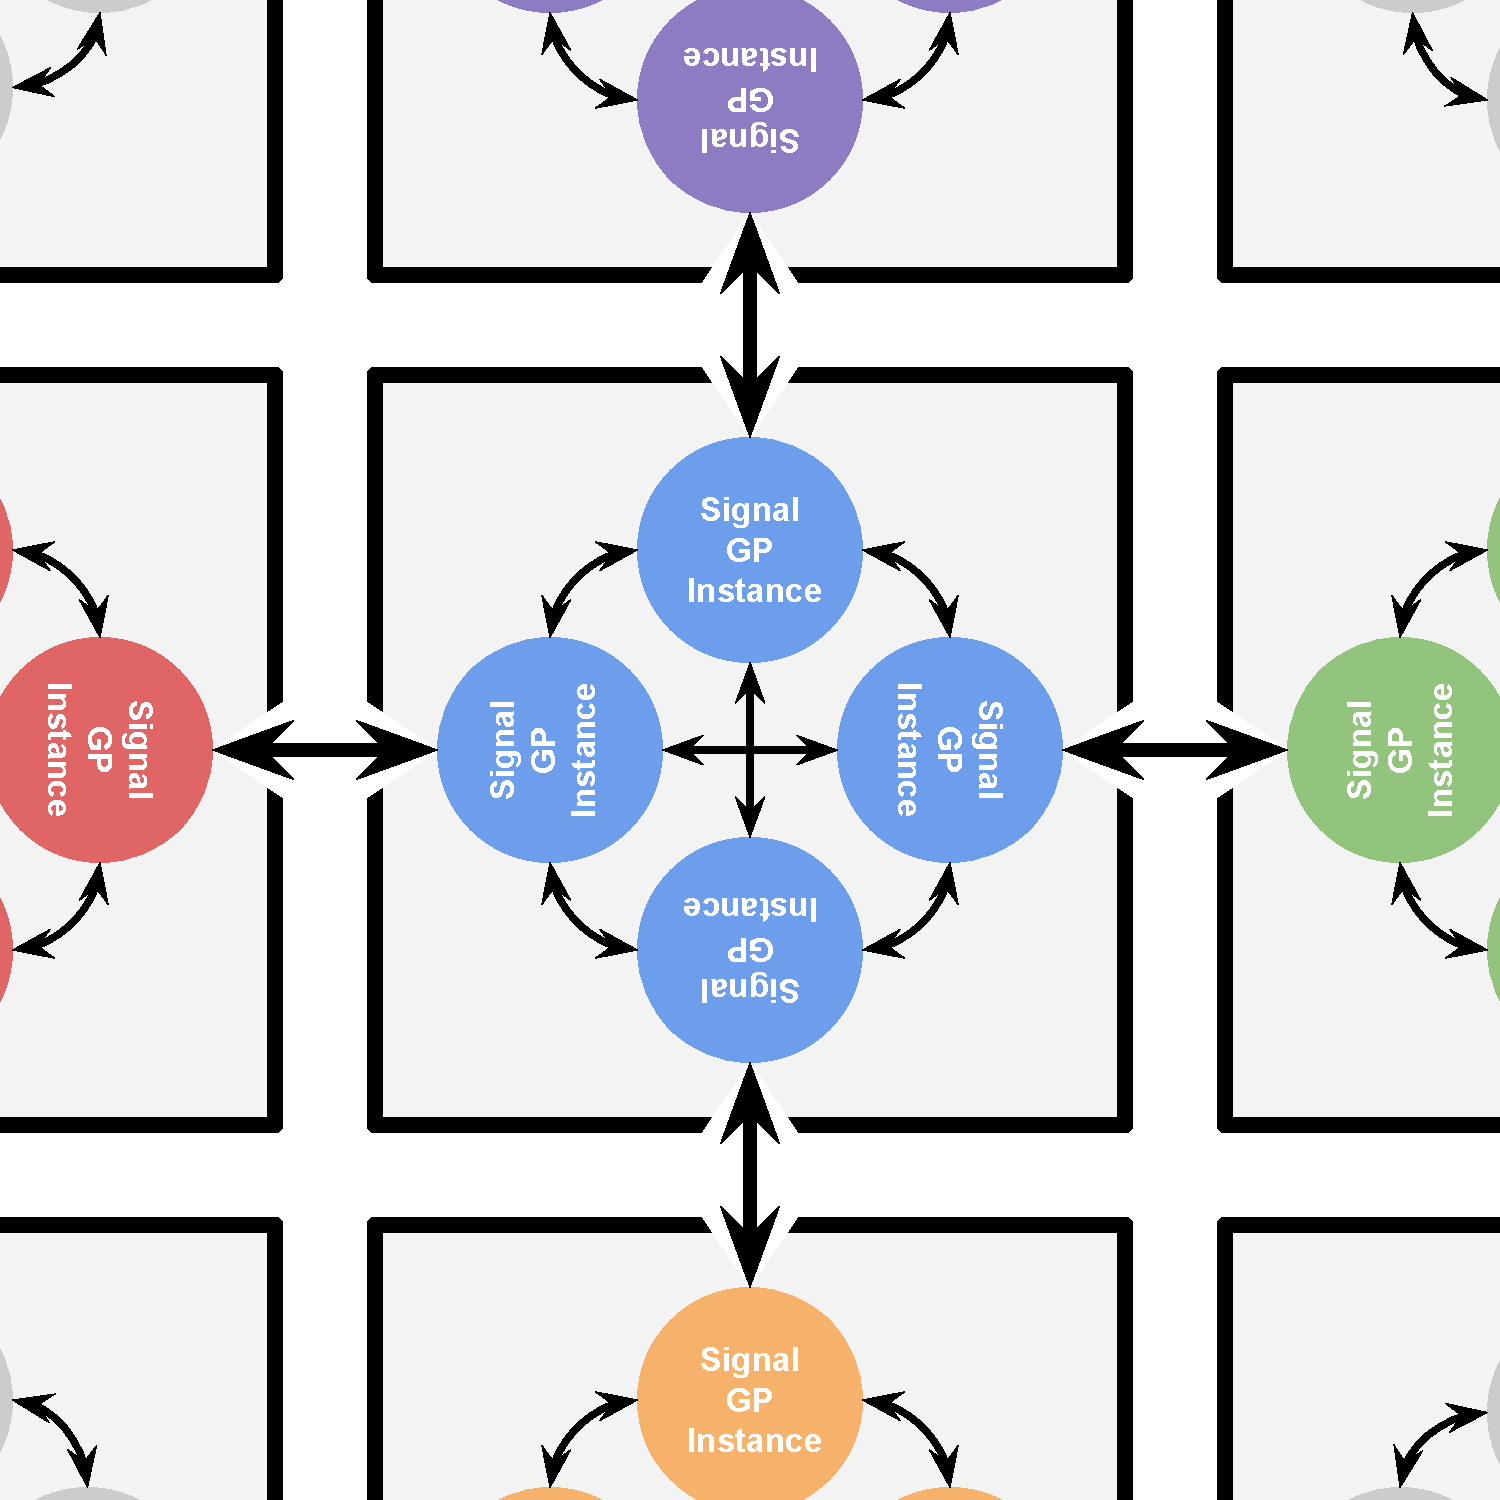
\includegraphics[width=\textwidth]{img/dishtinygp-cartoon}
\caption{
A cartoon overview of how individual SignalGP instances are organized into DISHTINY cells.
% Each cell contains four independent SignalGP instances.
% The same genetic program is mirrored across all four SignalGP instances, but each instance executes independently.
Within each DISHTINY cell, each of four independent instances senses environmental state, receives intercellular messages, and determines cell behavior with respect to a single cardinal direction.
All four instances sense non-directional environmental cues and non-directional actions may be taken by any instance.
Instances within a cell communicate via intracellular messaging.
}
\label{fig:dishtinygp-cartoon}
\end{subfigure}
\end{minipage}%
\hspace*{\fill}


\caption{
Schematic illustrations of how individual SignalGP instances function and how individual SignalGP instances are organized into DISHTINY cells.
Figure \ref{fig:signalgp-cartoon} provided courtesy Alexander Lalejini.
}
\label{fig:signalgp-dishtinygp}
\end{center}
\end{figure}


Our experiments used cell-level digital organisms controlled by evolving
genetic programs.
We employ the SignalGP representation, which expresses function-like modules of linear program instruction sequences in response to stimuli.
This event-driven paradigm facilitates the evolution of dynamic interactions between digital organisms and their environment (including other digital organisms) \cite{lalejini2018evolving}.

Previous work evolving digital organisms in grid-based problem domains has relied on a single computational instance which designates a direction to act in via an explicit cardinal ``facing'' state or output \cite{goldsby2014evolutionary, goldsby2018serendipitous, grabowski2010early, biswas2014causes, lalejini2018evolving}.
We introduce novel methodology that aims to facilitate the evolution of directionally symmetric phenotypes which effectively incorporate directionally-specific state.
In this work, each cell employs four instances of SignalGP hardware: one ``facing'' each cardinal direction.
These computational instances all execute the same SignalGP program but are otherwise decoupled and may follow independent chains of execution and develop independent regulatory states.
Instances within a cell may coordinate via so-called intracellular messaging.
Figure \ref{fig:dishtinygp-cartoon} schematically depicts the configuration of the four SignalGP instances that constitute a single DISHTINY cell as well as the instances of neighboring cells that receive extracellular messages from the focal cell.

\subsection{Treatments}

We screened evolutionary replicates conducted under combinations of two experimental conditions:
\begin{enumerate}
\item flat versus nested hierarchical resource wave/channel-signaling levels and
\item cooperative versus independent resource collection.
\end{enumerate}

The first experimental manipulation explores the effects of hierarchical nesting of kin-sensing and/or functional cooperation.
The second manipulation explores the effects of functional cooperation.

We mix and match these experimental manipulations in three treatments:
\begin{enumerate}
\item one level with even resource (``Flat-Even''; in-browser simulation \url{https://mmore500.com/hopto/i}),
\item one level with wave-based resource (``Flat-Wave''; in-browser simulation \url{https://mmore500.com/hopto/j}),
\item two levels with even resource (``Nested-Even''; in-browser simulation \url{https://mmore500.com/hopto/k}), and
\item two levels with wave-based resource (``Nested-Wave''; in-browser simulation \url{https://mmore500.com/hopto/l}).
\end{enumerate}
